\chapter{RESULTS}
\label{RESULTS}

\section{Results}
The results for the loss of weight are listed in table and in figure.


%{PhysRevC.69.065501, PhysRevLett.82.1096, PhysRevLett.96.022003, Aniol2006275, PhysRevLett.98.032301, PhysRevLett.108.102001, Spayde200479, PhysRevLett.92.102003, PhysRevLett.95.092001, PhysRevLett.104.012001, PhysRevLett.93.022002, PhysRevLett.94.152001, PhysRevLett.102.151803, PhysRevD.86.010001, PhysRevLett.109.203003, Wood21031997, PhysRevLett.111.141803}

\begin{singlespace}
\begin{figure}[!h]
	\begin{center}
	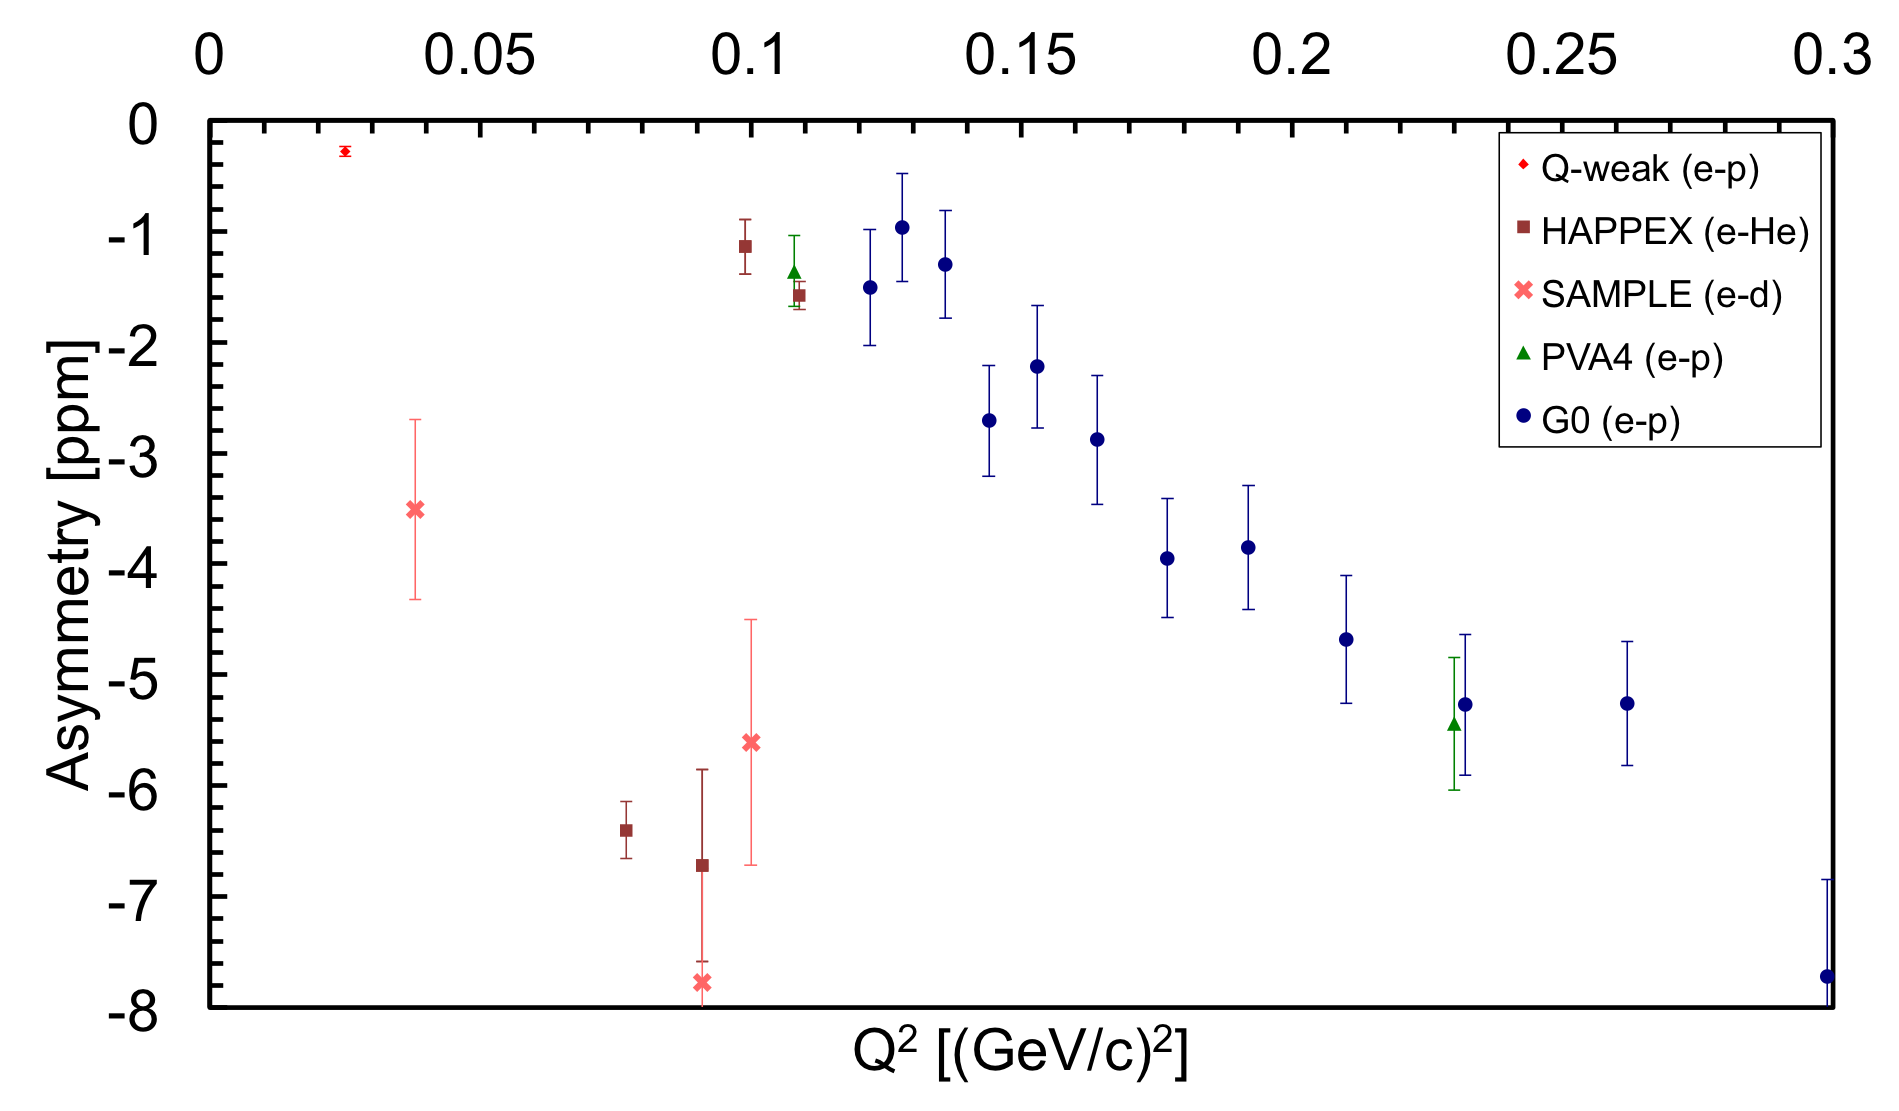
\includegraphics[width=15.0cm]{figures/qweak_asymmetry_zoomed}
	\end{center}
	\caption
	[Asymmetry obtained from the commissioning dataset of the Q-weak and PVES experiments.]
	{(Color online) Asymmetry obtained from the commissioning dataset of the Q-weak and PVES experiments up to $Q^{2}$ = 0.63~$(GeV/c)^{2}$~\cite{PhysRevC.69.065501, PhysRevLett.82.1096, PhysRevLett.96.022003, Aniol2006275, PhysRevLett.98.032301, PhysRevLett.108.102001, Spayde200479, PhysRevLett.92.102003, PhysRevLett.95.092001, PhysRevLett.104.012001, PhysRevLett.93.022002, PhysRevLett.94.152001, PhysRevLett.102.151803, PhysRevD.86.010001, PhysRevLett.109.203003, Wood21031997, PhysRevLett.111.141803} were used to extract $Q_{W}^{p}$. A zoomed asymmetry vs $Q^{2}$ is shown here for better visualization. The measured absolute asymmetry and uncertainty from this measurement are $\sim$3 times smaller than the previous PVES measurements.}
	\label{fig:qweak_asymmetry_zoomed}
\end{figure}
\end{singlespace}


\begin{singlespace}
\begin{figure}[!h]
	\begin{center}
	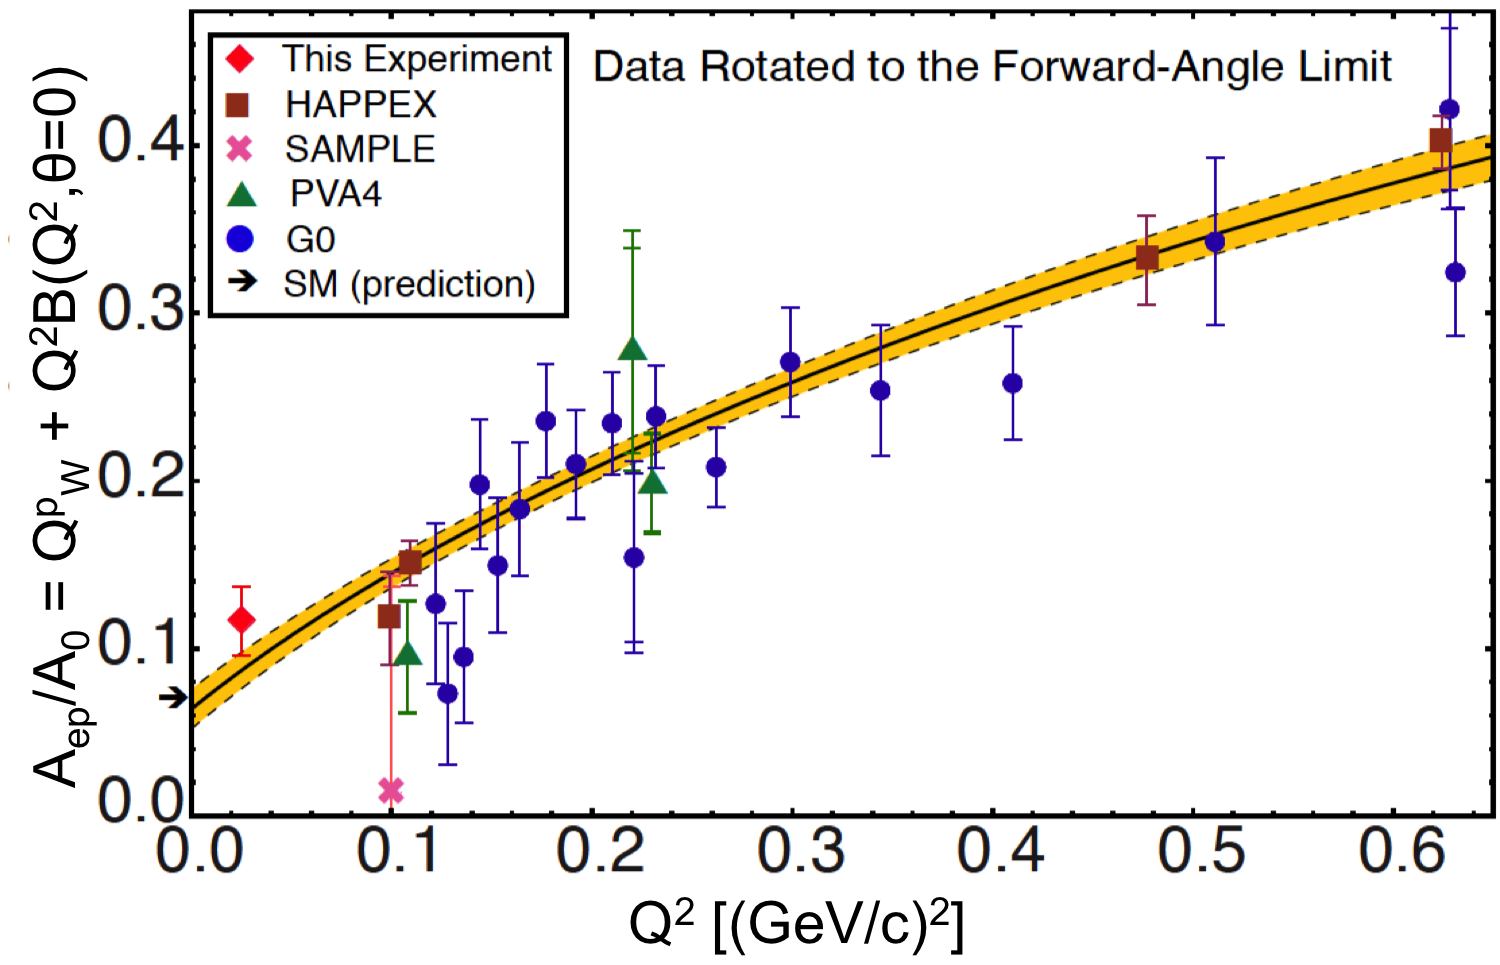
\includegraphics[width=15.0cm]{figures/qweakResult25Percent}
	\end{center}
	\caption
	[First result from Q-weak.]
	{(Color online) Global fit result (solid line) presented in the forward angle limit as reduced asymmetries derived from this measurement as well as other PVES experiments up to $Q^{2}$ = 0.63~$(GeV/c)^{2}$ \cite{PhysRevC.69.065501, PhysRevLett.82.1096, PhysRevLett.96.022003, Aniol2006275, PhysRevLett.98.032301, PhysRevLett.108.102001, Spayde200479, PhysRevLett.92.102003, PhysRevLett.95.092001, PhysRevLett.104.012001, PhysRevLett.93.022002, PhysRevLett.94.152001, PhysRevLett.102.151803, PhysRevD.86.010001, PhysRevLett.109.203003, Wood21031997, PhysRevLett.111.141803}, including proton, helium, and deuterium data. The additional uncertainty arising from this rotation is indicated by outer error bars on data points. The band indicates the uncertainty in the fit. $Q^{p}_{W}$ is the intercept of the fit. The SM prediction \cite{PhysRevD.86.010001} is also shown (arrow).}
	\label{fig:qweakResult25Percent}
\end{figure}
\end{singlespace}


\begin{singlespace}
\begin{figure}[!h]
	\begin{center}
	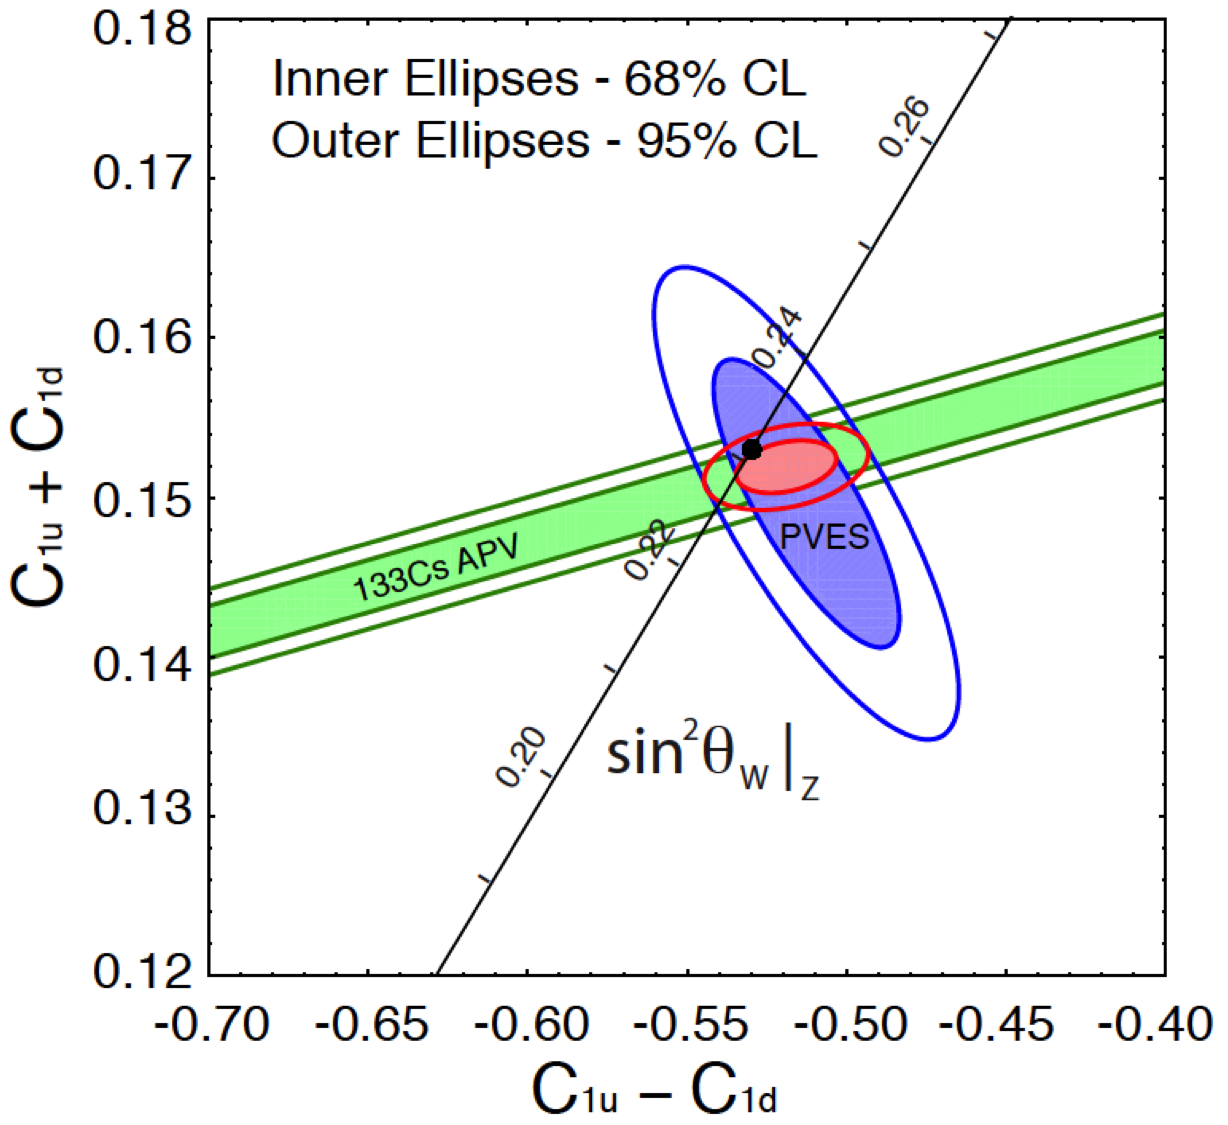
\includegraphics[width=12.0cm]{figures/qweakQuarkCouplings}
	\end{center}
	\caption
	[C1couplings with Qweak First Results.]
	{(Color online) Constraints on the neutral-weak quark coupling constants {$C_{1u}- C_{1d}$} (isovector) and {$C_{1u} + C_{1d}$} (isoscalar). The near horizontal (green) APV band constrains the isoscalar combination from $^{133}$Cs data~\cite{PhysRevLett.109.203003, Wood21031997}. The vertical (blue) ellipse  represents the global fit of the existing $Q^2 \textless 0.63$ $(GeV/c)^{2}$ PVES data~\cite{PhysRevC.69.065501, PhysRevLett.82.1096, PhysRevLett.96.022003, Aniol2006275, PhysRevLett.98.032301, PhysRevLett.108.102001, Spayde200479, PhysRevLett.92.102003, PhysRevLett.95.092001, PhysRevLett.104.012001, PhysRevLett.93.022002, PhysRevLett.94.152001, PhysRevLett.102.151803, PhysRevD.86.010001, PhysRevLett.109.203003, Wood21031997, PhysRevLett.111.141803} including the new result reported here at $Q^{2}$=0.025 $(GeV/c)^{2}$. The small (red) ellipse near the center of the figure shows the result obtained by combining the APV and PVES information. The SM prediction~\cite{PhysRevD.86.010001} as a function of $\sin^{2}\theta_W $ in the $\overline{MS}$ scheme is plotted (diagonal black line) with the SM best fit value indicated by the (black) point at $\sin^{2}\theta_W $=0.23116.}
	\label{fig:qweakQuarkCouplings}
\end{figure}
\end{singlespace}


\subsection{Modeling Copy2}
